\chapter{Length}
 
Recall that a sequence 
\[a=t_0 < t_1 < \cdots < t_k=b.\]
is called a \emph{partition} of the interval $[a,b]$.

\begin{thm}{Definition}\label{def:length}
Let $\alpha\:[a,b]\to \mathcal{X}$ be a curve in a metric space.
The \emph{length}\index{length of curve} of a $\alpha$ is defined as
\begin{align*}
\length \alpha
= 
\sup \{|\alpha(t_0)-\alpha(t_1)|&+|\alpha(t_1)-\alpha(t_2)|+\dots
\\
&\dots+|\alpha(t_{k-1})-\alpha(t_k)|\},
\end{align*}
where the exact upper bound is taken over all partitions
\[a=t_0 < t_1 < \cdots < t_k=b.\]

The length of $\alpha$ is a nonnegative real number or infinity;
the curve $\alpha$ is called \emph{rectifiable}\index{rectifiable curve} if its length is finite. 

The length of a closed curve is defined as the length of a corresponding loop.
If a curve is defined on a open or closed-open interval then its length is defined as the exact upper bound for lengths of all its closed arcs.
\end{thm}

If $\alpha$ is a space curve, then the above definition says that it length is the exact upper bound of the lengths of polygonal lines $p_0\dots p_k$ \emph{inscribed} in the curve, where $p_i=\alpha(t_i)$ for a  partition $a=t_0 < t_1 < \cdots < t_k=b$.
If $\alpha$ is closed then $p_0=p_k$ and therefore the inscribed polygonal line is also closed.

\begin{thm}{Exercise}\label{ex:integral-length}
Assume $\alpha\:[a,b]\to\RR^2$ is a smooth curve.
Show that
\begin{enumerate}[(a)]
\item\label{ex:integral-length>} $\length \alpha\ge \int_a^b|\alpha'(t)|\cdot dt$,
\item\label{ex:integral-length<} $\length \alpha\le \int_a^b|\alpha'(t)|\cdot dt$.
\end{enumerate}
Conclude that 
\[\length \alpha= \int_a^b|\alpha'(t)|\cdot dt.\]
\end{thm}

\parit{Hints:} For (\ref{ex:integral-length>}), apply the fundamental theorem of calculus for each segment in a given partition. For (\ref{ex:integral-length<}) consider a partition such that the velocity vector $\alpha'(t)$ is nearly constant on each of its segments.

\parbf{Nonrectifiable curves.}
A classical example of a nonrectifiable curve is the so called \emph{Koch snowflake};
it is a fractal curve that can be constructed the following way:

Start with an equilateral triangle, divide each of its side into three segments of equal length and add an equilateral triangle with base at the middle segment.
Repeat this construction recursively to the obtained polygons.
\begin{figure}[h!]
\begin{minipage}{.24\textwidth}
\centering
\vskip5.9mm
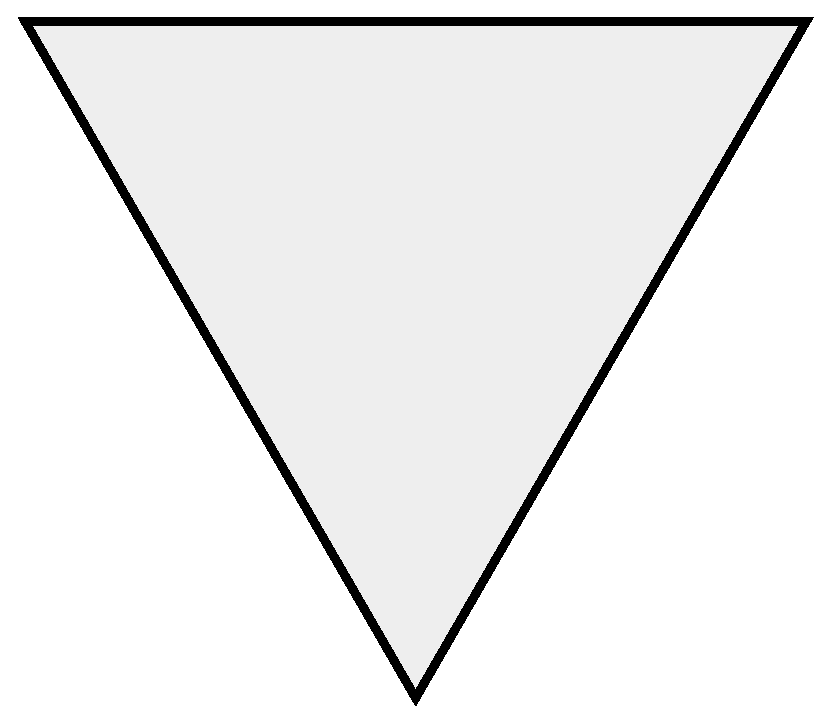
\includegraphics[scale=.15]{pics/Koch_Snowflake-0}
\end{minipage}
\hfill
\begin{minipage}{.24\textwidth}
\centering
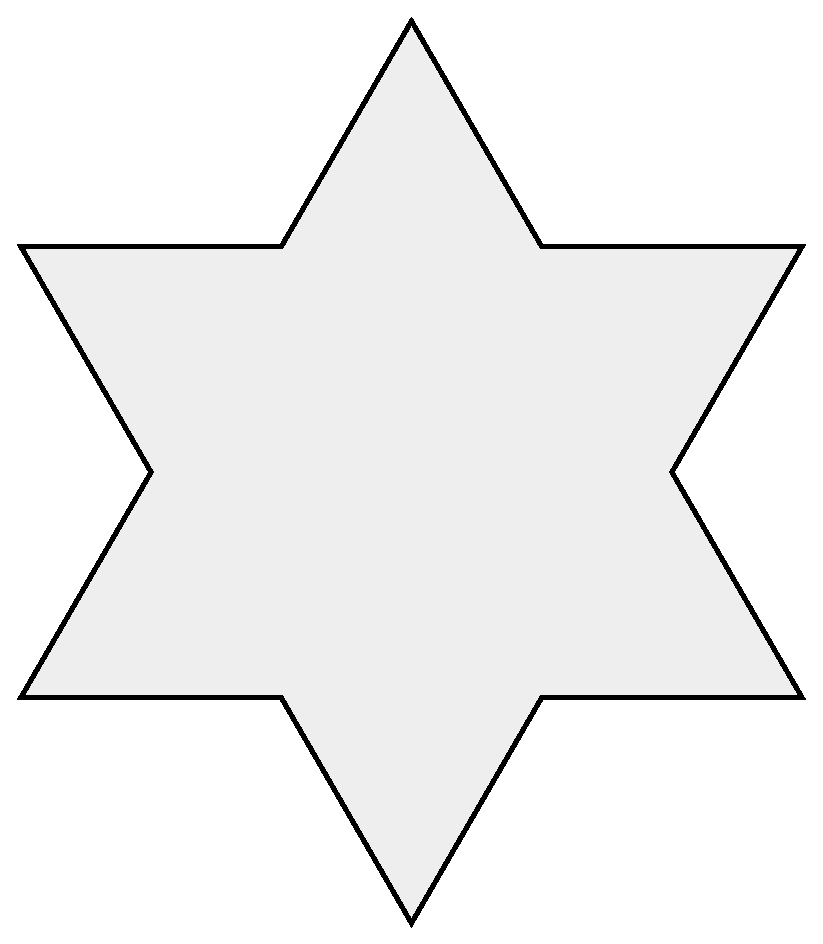
\includegraphics[scale=.15]{pics/Koch_Snowflake-1}
\end{minipage}
\hfill
\begin{minipage}{.24\textwidth}
\centering
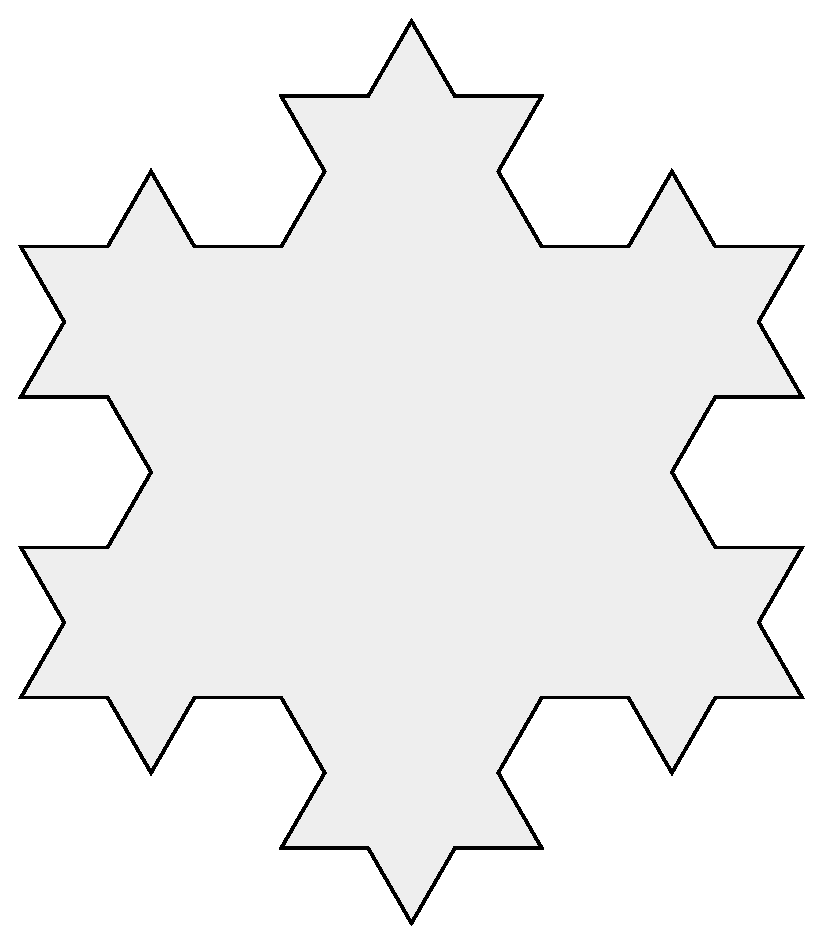
\includegraphics[scale=.15]{pics/Koch_Snowflake-2}
\end{minipage}
\hfill
\begin{minipage}{.24\textwidth}
\centering
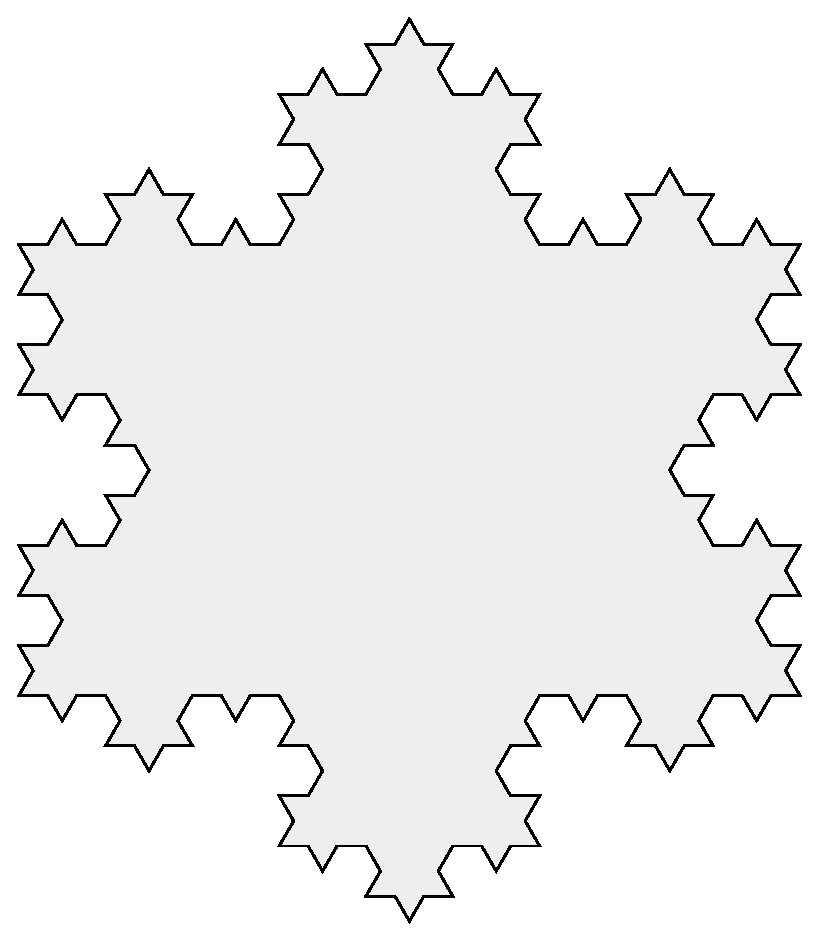
\includegraphics[scale=.15]{pics/Koch_Snowflake-3}
\end{minipage}
\end{figure}
Few first iterations of the construction are shown on the diagram.
The Koch snowflake is the boundary of the union of all the polygons.


\begin{thm}{Exercise}\label{ex:nonrectifiable-curve}
\begin{enumerate}[(a)]
\item Show that Koch snowflake is a closed simple curve; that is, it admits a homeomorphism to a circle.
\item\label{ex:nonrectifiable-curve:b} Show that Koch snowflake is not rectifiable. 
\end{enumerate}
\end{thm}

\section*{Arc length parametrization}

We say that a parametrized curve $\gamma$ has an \emph{arc length parametrization}\footnote{which is also called \emph{natural parametrization}}
if for any two values of parameters $t_1<t_2$, the value $t_2-t_1$ is the length of $\gamma|_{[t_1,t_2]}$; that is, the closed arc of $\gamma$ from $t_1$ to $t_2$.

Note that a smooth space curve $\gamma(t)=(x(t),y(t),z(t))$ has arc length parametrization if and only if it has unit velocity vector at all times;
that is 
\[|\gamma'(t)|=\sqrt{x'(t)^2+y'(t)^2+z'(t)^2}=1;\]
by that reason arc length parametrization of smooth curves with also called \emph{unit-speed curves}.
Note that smooth unit-speed curves are automatically regular.


Any rectifiable curve can be parameterized by arc length.
For a parametrized smooth curve $\gamma$, the arc length parameter $s$ can be written as an integral
\[s(t)=\int_{t_0}^t |\gamma'(\tau)|\cdot d\tau.\]
Note that $s(t)$ is a smooth increasing function.
Further by fundamental theorem of calculus, $s'(t)=|\gamma'(t)|$.
Therefore if $\gamma$ is regular, then $s'(t)\ne0$ for any parameter value $t$.
By inverse function theorem (\ref{thm:inverse}) the inverse function $s^{-1}(t)$ is also smooth.
Therefore after the reparametrization of $\gamma$ by arclength  $s$ it remains smooth and regular.

We will be interested in the properties of curves that are invariant under a reparametrization.
Therefore we can always assume that the given smooth regular curve comes with a arc length parametrization.
A good property of arc length parametrizations is that it is almost canonical --- these parametrizations differ only by a sign and additive constant.
On the other hand, often it is impossible to find an arc length parametrization in a closed form which makes it hard to use it calculations;
usually it is more convenient to use the original parametrization.

\begin{thm}{Exercise}\label{ex:arc-length-helix}
Reparametrize the helix 
$\gamma_a(t)=(a\cdot\cos t,a\cdot \sin t,t)$
by arc length.
\end{thm}



\section*{Convex curves}

A closed simple plane curve is called \emph{convex} if it bounds a convex region.

\begin{thm}{Proposition}\label{prop:convex-curve}
Assume a convex curve $\alpha$ lies inside the domain bounded by a closed simple plane curve $\beta$.
Then
\[\length\alpha\le \length\beta.\]
\end{thm}

Note that it is sufficient to show that for any polygon  $P$ inscribed in $\alpha$ there is a polygon $Q$ inscribed in $\beta$ with 
$\perim P\le \perim Q$, where $\perim P$ denotes the perimeter of $P$.

Therefore it is sufficient to prove the following lemma.


\begin{thm}{Lemma}\label{lem:perimeter}
Let $P$ and $Q$ be polygons.
Assume $P$ is convex and $Q\supset P$.
Then 
\[\perim P\le \perim Q.\]

\end{thm}


\begin{wrapfigure}{r}{24 mm}
\vskip-4mm
\centering
\includegraphics{mppics/pic-7}
%\caption*{}
\end{wrapfigure}

\parit{Proof.}
Note that by the triangle inequality,
the inequality
\[\perim P\le \perim Q\]
holds
if $P$ can be obtained from $Q$ by cutting it along a chord;
that is, a line segment with ends on the boundary of $Q$ that lies in $Q$.


Note that there is an increasing sequence of polygons 
$$P=P_0\subset P_1\subset\dots\subset P_n=Q$$
such that $P_{i-1}$ obtained from $P_{i}$ by cutting along a chord.
Therefore 
\begin{align*}
\perim P=\perim P_0&\le\perim P_1\le\dots
\\
\dots&\le\perim P_n=\perim Q
\end{align*}
and the lemma follows.
\qeds

\begin{thm}{Corollary}
Any convex closed plane curve is rectifiable.  
\end{thm}

\parit{Proof.}
Any closed curve is bounded; that is, it lies in a sufficiently large square.
Indeed the curve can be described as an image of a loop $\alpha\:[0,1]\to\RR^2$, $\alpha(t)=(x(t),y(t))$.
The coordinate functions $x(t)$ and $y(t)$ are continous functions defined on $[0,1]$.
Therefore the absolute values of both of these functions are bounded by some constant $C$.
That is $\alpha$ lies in the square defined by the inequalities $|x|\le C$ and $|y|\le C$.

By Proposition~\ref{prop:convex-curve}, the length of the curve can not exceed the perimeter of the square $8\cdot C$, whence the result.
\qeds

Recall that convex hull of a set $X$ is the smallest convex set that contains $X$; in other words convex hull is the intersection of all convex sets containing $X$.

\begin{thm}{Exercise}\label{ex:convex-hull}
Let $\alpha$ be a closed simple plane curve.
Denote by $K$ the convex hull of $\alpha$; let $\beta$ be the boundary curve of $X$.
Show that 
\[\length \alpha\ge \length \beta.\]

Try to show that the statement holds for arbitrary closed plane curve $\alpha$, assuming that $X$ has nonempty interior.
\end{thm}




\section*{Semicontinuity of length}

Recall that the lower limit 
of a sequence of real numbers $(x_n)$ is denoted by
\[\liminf_{n\to\infty} x_n.\] 
It is defined as the lowest partial limit; that is, the lowest possible limit of a subsequence of $(x_n)$.
The lower limit is defined for any sequence of real numbers and it lies in the exteded real line $[-\infty,\infty]$


\begin{thm}{Theorem}\label{thm:length-semicont}
Length is a lower semi-continuous with respect to pointwise convergence of curves. 

More precisely, assume that a sequence
of curves $\alpha_n\:[a,b]\to \spc{X}$ in a metric space $\spc{X}$ converges pointwise 
to a curve $\alpha_\infty\:[a,b]\to \spc{X}$;
that is, $\alpha_n(t)\z\to\alpha_\infty(t)$ for any fixed $t\in[a,b]$ as $n\to\infty$. 
Then 
$$\liminf_{n\to\infty} \length\alpha_n \ge \length\alpha_\infty.\eqlbl{eq:semicont-length}$$
\end{thm}



\begin{wrapfigure}{r}{20 mm}
\vskip-0mm
\centering
\includegraphics{mppics/pic-6}
\end{wrapfigure}


Note that the inequality \ref{eq:semicont-length} might be strict.
For example the diagonal $\alpha_\infty$ of the unit square 
can be  approximated by a sequence of stairs-like
polygonal curves $\alpha_n$
with sides parallel to the sides of the square ($\alpha_6$ is on the picture).
In this case
\[\length\alpha_\infty=\sqrt{2}\quad
\text{and}\quad \length\alpha_n=2\]
for any $n$.

\parit{Proof.}
Fix a partition $a=t_0<t_1<\dots<t_k=b$.
Set 
\begin{align*}\Sigma_n
&\df
|\alpha_n(t_0)-\alpha_n(t_1)|+\dots+|\alpha_n(t_{k-1})-\alpha_n(t_k)|.
\\
\Sigma_\infty
&\df
|\alpha_\infty(t_0)-\alpha_\infty(t_1)|+\dots+|\alpha_\infty(t_{k-1})-\alpha_\infty(t_k)|.
\end{align*}

Note that $\Sigma_n\to \Sigma_\infty$ as $n\to\infty$
and $\Sigma_n\le\length\alpha_n$ for each $n$.
Hence
$$\liminf_{n\to\infty} \length\alpha_n \ge \Sigma_\infty.\eqlbl{>=Sigma-infty}$$

If $\alpha_\infty$ is rectifiable, we can assume that 
\begin{align*}
\length\alpha_\infty<\Sigma_\infty+\eps.
\end{align*}
for any given $\eps>0$.
By \ref{>=Sigma-infty} it follows that 
$$\liminf_{n\to\infty} \length\alpha_n > \length\alpha_\infty-\eps$$
for any $\eps>0$; whence \ref{eq:semicont-length} follows.

It remains to consider the case when $\alpha_\infty$ is not rectifiable; 
that is $\length\alpha_\infty=\infty$.
In this case we can choose a partition so that $\Sigma_\infty>L$ for any real number $L$.
By \ref{>=Sigma-infty} it follows that 
$$\liminf_{n\to\infty} \length\alpha_n > L$$
for any $L$; whence $\liminf_{n\to\infty}=\infty$ and \ref{eq:semicont-length} follows.
\qeds

\section*{Length metric}

Let $\spc{X}$ be a metric space.
Given two points $x,y$ in $\spc{X}$, denote by $d(x,y)$ the exact lower bound for lengths of all paths connecting $x$ to $y$; if there is no such path we assume that $d(x,y)=\infty$.

Note that function $d$ satisfies all the axioms of metric except it might take infinite value.
Therefore if any two points in $\spc{X}$ can be connected by a rectifiable curve, then $d$ defines a new metric on $\spc{X}$; in this case $d$ is called \emph{induced length metric}.

Evidently $d(x,y)\ge |x-y|$ for any pair of points $x,y\in \spc{X}$.
If the equality holds for any pair, then then the metric is called \emph{length metric} and the space is called \emph{length-metric space}.

Most of the time we consider length-metric spaces.
In particular the Euclidean space is a length-metric space.
A subspaces $A$ of length-metric space $\spc{X}$ might be not a lenght-metric space;
the induced length distance between points $x$ and $y$ in the subspace $A$ will be denoted as $|x-y|_A$;
that is $|x-y|_A$ is the exact lower bound for the length of paths in $A$.

\begin{thm}{Exercise}\label{ex:intrinsic-convex}
Let $A\subset \RR^3$ be a closed subset.
Show that $A$ is convex if and only if
\[|x-y|_A=|x-y|_{\RR^3}.\]
\end{thm}

\begin{thm}{Exercise}\label{ex:S1-intrinsic}
Let us denote by $\SS^1$ the unit circle in the plane; that is,
\[\SS^1=\set{(x,y)\in\RR^3}{x^2+y^2=1}.\]
Show that
\[|u-v|_{\SS^1}=\measuredangle(u,v)\df\arccos\langle u,v\rangle\]
for any $u,v\in \SS^1$.
\end{thm}

\section*{Spherical curves}

\begin{thm}{Exercise}\label{ex:S2-intrinsic}
Let us denote by $\SS^2$ the unit sphere in the space; that is,
\[\SS^2=\set{(x,y,z)\in\RR^3}{x^2+y^2+z^2=1}.\]
Show that
\[|u-v|_{\SS^2}=\measuredangle(u,v)\df\arccos\langle u,v\rangle\]
for any $u,v\in \SS^2$.
\end{thm}

\parit{Hint:} Use Exercise~\ref{ex:S1-intrinsic} and the following map $f\:(r,\theta,\phi)\mapsto (r,\theta,0)$ in spherical coordinates. Note that $f$ is distance nonexpanding and it maps $\RR^3$ to a half-plane and $\SS^2$ to one of its meridians.

\begin{thm}{Hemisphere lemma}
\label{lem:hemisphere}
Any closed curve of length $<2\cdot \pi$ in $\SS^2$ lies in an open hemisphere. 
\end{thm}

\parit{Proof.}
Let $\alpha$ be a closed curve in $\mathbb{S}^2$ of length $2\cdot\ell$.

%???+PIC

Assume $\ell<\pi$.

\begin{wrapfigure}{r}{35 mm}
\vskip-0mm
\centering
\includegraphics{mppics/pic-52}
\caption*{The north hemisphere corresponds to the disc and the south hemisphere to the complement of the disc.}
\end{wrapfigure}

Let us divide $\alpha$ into two arcs $\alpha_1$ and $\alpha_2$ of length $\ell$, with endpoints $p$ and $q$. 
According to Exercise~\ref{ex:S2-intrinsic}, $\measuredangle(p,q)\le\ell<\pi$.
Denote by $z$ be the midpoint between $p$ and $q$ in $\mathbb{S}^2$;
that is $z$ is the midpoint of an equator arc from $p$ to $q$. 
We claim that $\alpha$ lies in the open north hemisphere with north pole at $z$.  
If not, $\alpha$ intersects the equator in a point, say $r$.
Without loss of generality we may assume that $r$ lies on~$\alpha_1$. 

Rotate the arc $\alpha_1$ by angle $\pi$ around the line thru $z$ and the center of the sphere.
The obtained arc $\alpha_1^{*}$ together with $\alpha_1$ forms a closed curve of length $2\cdot \ell$ that passes thru $r$ and its antipodal point $r^{*}$.
Therefore
\[\tfrac12\cdot\length \alpha=\ell\ge \measuredangle(r,r^{*})=\pi,\] 
a contradiction.
\qeds

\begin{thm}{Exercise}\label{ex:flaw}
Consider the following problem, find a flaw in the given wrong solution.
Come up with a correct argument.
\end{thm}

 
\parbf{Problem.}
Suppose that a closed plane curve $\alpha$ has length at most 4.
Show that $\alpha$ lies in a unit disc.

\parit{Wrong solution.}
Note that it is sufficient to show that diameter of $\alpha$ is at most 2;
that is, the distance between any two pairs of points $p$ and $q$ of $\alpha$ an not exceed $2$.

The length of $\alpha$ can not be smaller then the closed inscribed polygonal line which goes from $p$ to $q$ and back to $p$.
Therefore 
\[2\cdot |p-q|\le\length \alpha\le 4.\]
\qedsf
